	\chapter{Количественные характеристики формирования спата в поселениях {\it Macoma balthica}  на литорали губы Чупа (Белое море)}
Для получения прямой информации о формировании спата в $2006$~году были проведены ограниченные наблюдения за поселениями в губе Чупа.
Было обследовано 2 участка на о.~Кереть: в Сухой салме и в бухте Клющиха, и 2 материковых участка: в бухте Лисья и в проливе Подпахта.

Обилие {\it Macoma balthica} на исследованных участках варьировало в значительных пределах. 
Так, численность на разных участках составляла от $228$ до $1230$~экз./м$^2$, а биомасса от $1,1$ до $6,2$~г/м$^2$ (табл.~\ref{tab:NMacoma_recruitment}). 
\begin{table}[p]
\caption{Характеристики обилия взрослых {\it Macoma balthica} и спата на участках в губе Чупа в 2006 году}
\label{tab:NMacoma_recruitment}
\begin{center}
\begin{tabular}{|l|cc|c|}
\hline
Участок         & $N_{ad}$  & $B_{ad}$   & $N_{juv}$ \\ \hline
Сухая салма     & 1230 (17) & 6,2 (19) & 4980 (13)  \\  
Бухта Лисья     & 1200 (17) & 1,9 (18) & 4040 (21)  \\ 
бухта Клющиха   & 476 (19)  & 1,1 (24) & 4240 (10)  \\  
пролив Подпахта & 228 (30)  & 1,8 (64) & 10060 (15) \\ \hline
\end{tabular}
\end{center}

\footnotesize{Примечание: $N_{ad}$ --- средняя численность взрослых маком в поселении,~экз./м$^2$; 
$B_{ad}$ --- средняя биомасса взрослых маком в поселении,~г/м$^2$; 
$N_{juv}$ --- средняя численность спата маком в поселении,~экз./м$^2$. 
В скобках приведена точность учета $d$ в процентах.}
\end{table}

Численность взрослых особей {\it M.~balthica} на участке в Сухой салме составляла $1230 \pm 207$~экз./м$^2$, а биомасса "--- $6,2 \pm 1,17$~г/м$^2$. 
На участке были представлены моллюски с раковиной длиной от $1,1$ до $15,7$~мм. 
Размерная структура в Сухой салме характеризовалась бимодальностью с модальными классами $1,1 - 2,0$~мм и $6,1 - 8,0$~мм (рис.~\ref{ris:Chupa_spat_sizestr}). 
	\begin{figure}[p]
	\begin{minipage}[b]{.46\linewidth}
	\begin{center}
	Взрослые особи
	\end{center}
	\end{minipage}
	%
	\hfil %Это пружинка отодвигающая рисунки друг от друга
	\begin{minipage}[b]{.46\linewidth}
	\begin{center}
	Спат (генерация 2006 года)
	\end{center}
	\end{minipage}
%
	\begin{minipage}[b]{\linewidth}
	\begin{center}
		Сухая салма
	\end{center}
	\end{minipage}
%
	\begin{minipage}[b]{.46\linewidth}
	%Фигурка в первом ряду слева размер отведенный под весь этот объект \textendash 0.46 от ширины строки
	%Параметр [b] означает, что выравнивание этих министраниц будет по нижнему краю
	\begin{center}
		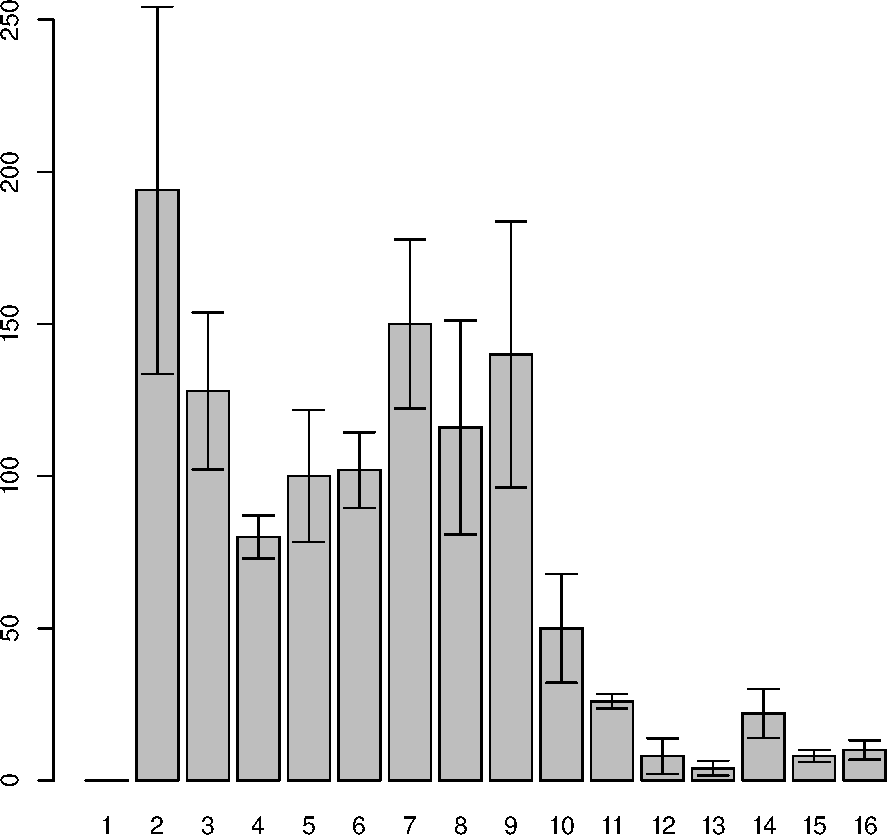
\includegraphics[width=0.21\textheight]{../White_Sea/spat/adult_str_Suhaya_1.pdf}
	\end{center}
	\end{minipage}
	%
	\hfil %Это пружинка отодвигающая рисунки друг от друга
	\begin{minipage}[b]{.46\linewidth}
%Следующий рисунок - первый ряд справа %DUNGEON S_4 \ AB
	\begin{center}
		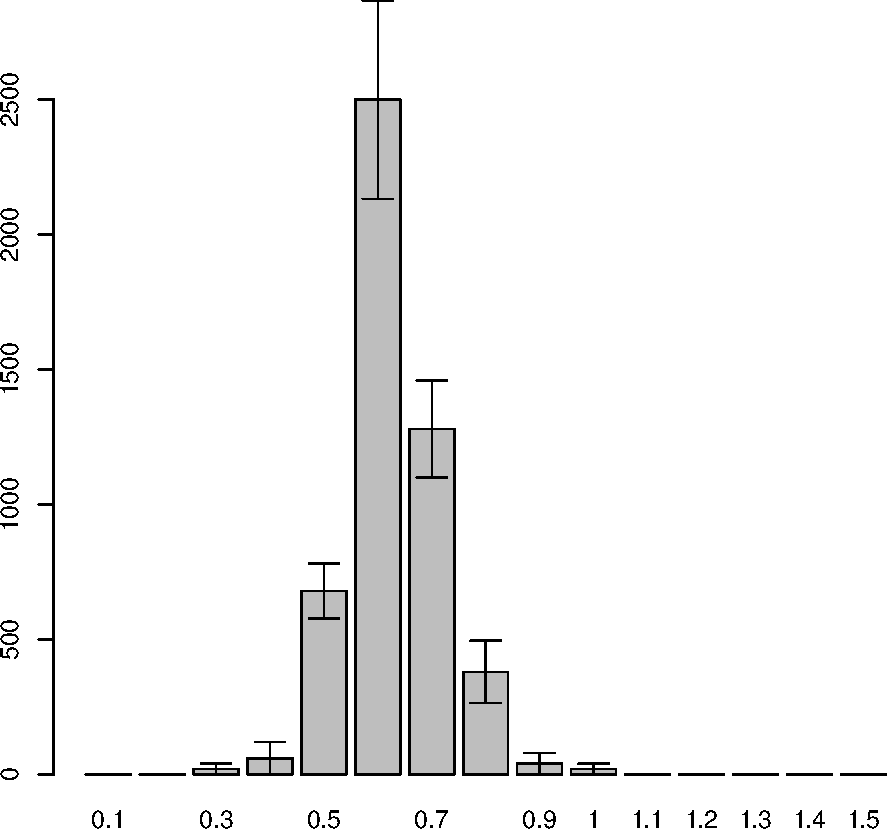
\includegraphics[width=0.21\textheight]{../White_Sea/spat/spat_str_Suhaya_1.pdf}
	\end{center}
	\end{minipage}
%\smallskip
%
	\begin{minipage}[b]{\linewidth}
	\begin{center}
		бухта Лисья
	\end{center}
	\end{minipage}
%
	\begin{minipage}[b]{.46\linewidth}
%Фигурка в первом ряду слева размер отведенный под весь этот объект \textendash 0.46 от ширины строки
%Параметр [b] означает, что выравнивание этих министраниц будет по нижнему краю
	\begin{center}
		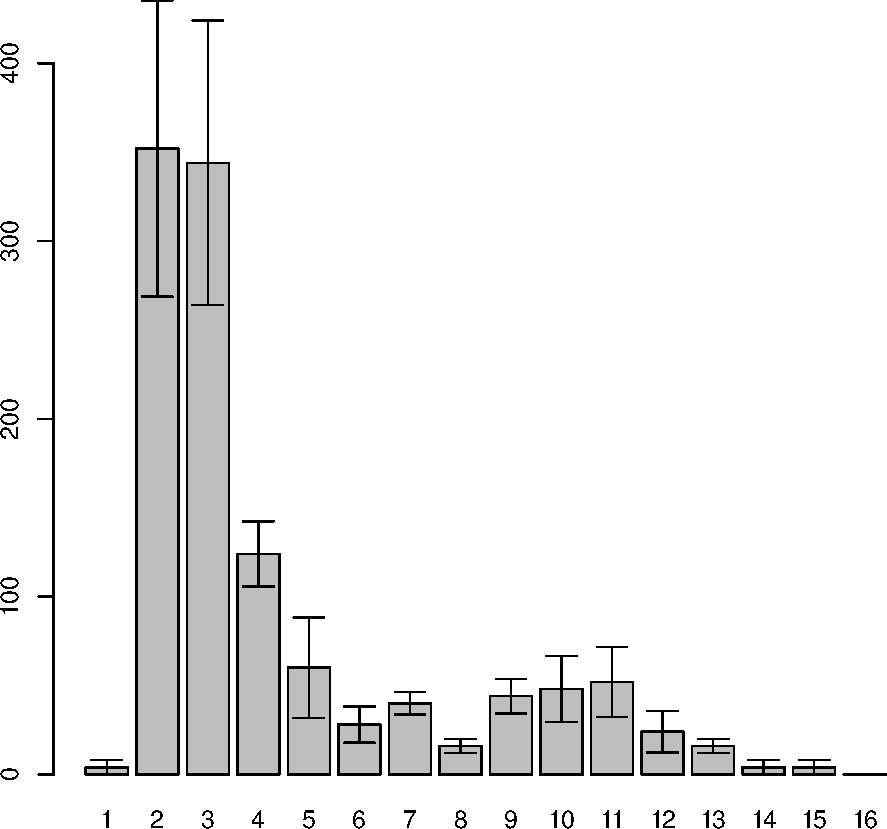
\includegraphics[width=0.215\textheight]{../White_Sea/spat/adult_str_Lisya_1.pdf}
	\end{center}
	\end{minipage}
%
	\hfil %Это пружинка отодвигающая рисунки друг от друга
%
	\begin{minipage}[b]{.46\linewidth}
%Следующий рисунок - первый ряд справа %DUNGEON S_4 \ AB
	\begin{center}	
		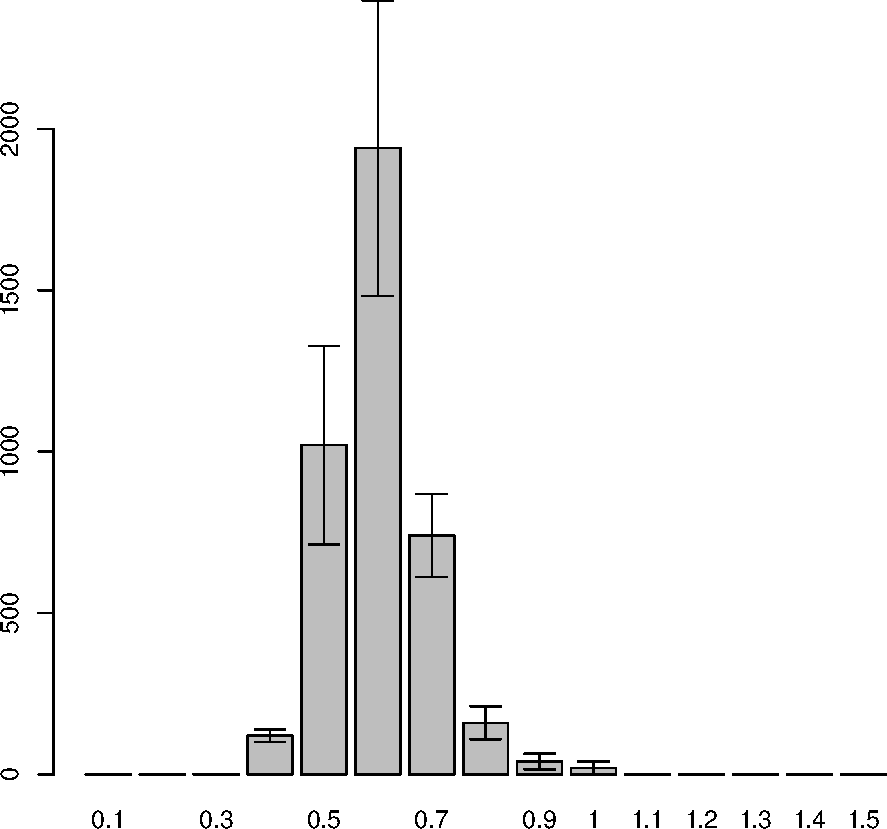
\includegraphics[width=0.215\textheight]{../White_Sea/spat/spat_str_Lisya_1.pdf}
	\end{center}
	\end{minipage}
%\smallskip
%
	\begin{minipage}[b]{\linewidth}
	\begin{center}
		бухта Клющиха
	\end{center}
	\end{minipage}
%
	\begin{minipage}[b]{.49\linewidth}
%Фигурка в первом ряду слева размер отведенный под весь этот объект \textendash 0.46 от ширины строки
%Параметр [b] означает, что выравнивание этих министраниц будет по нижнему краю
	\begin{center}
		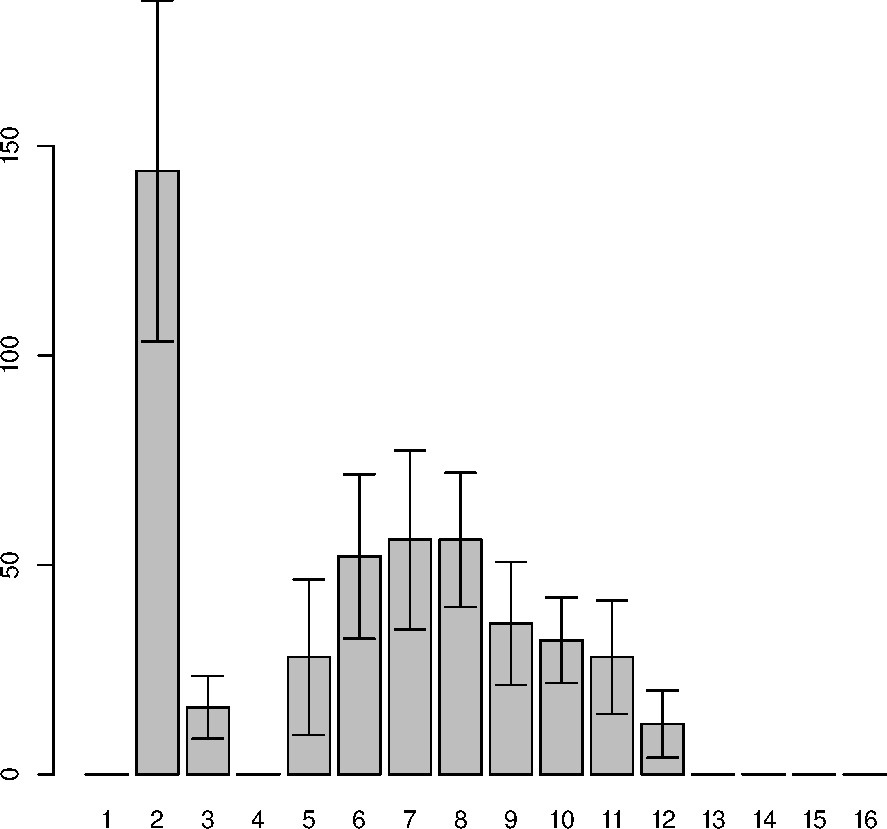
\includegraphics[width=0.215\textheight]{../White_Sea/spat/adult_str_Klushiha_1.pdf}
	\end{center}
	\end{minipage}
%
	\hfil %Это пружинка отодвигающая рисунки друг от друга
%
	\begin{minipage}[b]{.49\linewidth}
%Следующий рисунок - первый ряд справа %DUNGEON S_4 \ AB
	\begin{center}	
		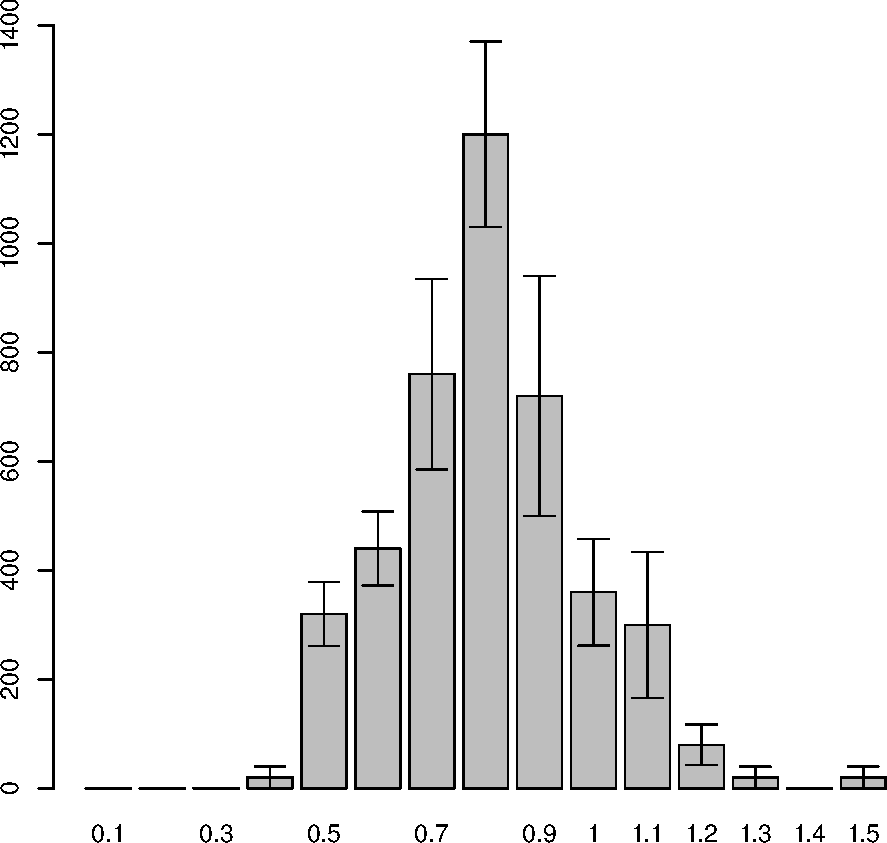
\includegraphics[width=0.215\textheight]{../White_Sea/spat/spat_str_Klushuha_1.pdf}
	\end{center}
	\end{minipage}
%\smallskip
%
	\begin{minipage}[b]{\linewidth}
	\begin{center}
		пролив Подпахта
	\end{center}
	\end{minipage}
%
	\begin{minipage}[b]{.49\linewidth}
%Фигурка в первом ряду слева размер отведенный под весь этот объект \textendash 0.46 от ширины строки
%Параметр [b] означает, что выравнивание этих министраниц будет по нижнему краю
	\begin{center}
		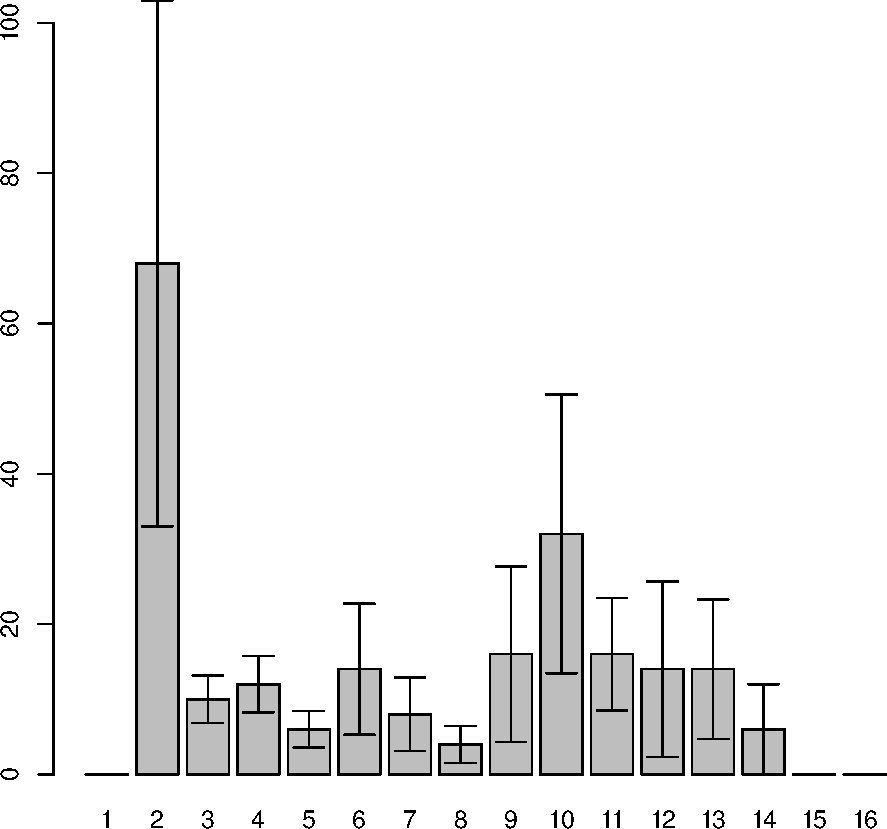
\includegraphics[width=0.215\textheight]{../White_Sea/spat/adult_str_Podpahta_1.pdf}
	\end{center}
	\end{minipage}
%
	\hfil %Это пружинка отодвигающая рисунки друг от друга
%
	\begin{minipage}[b]{.49\linewidth}
%Следующий рисунок - первый ряд справа %DUNGEON S_4 \ AB
	\begin{center}	
		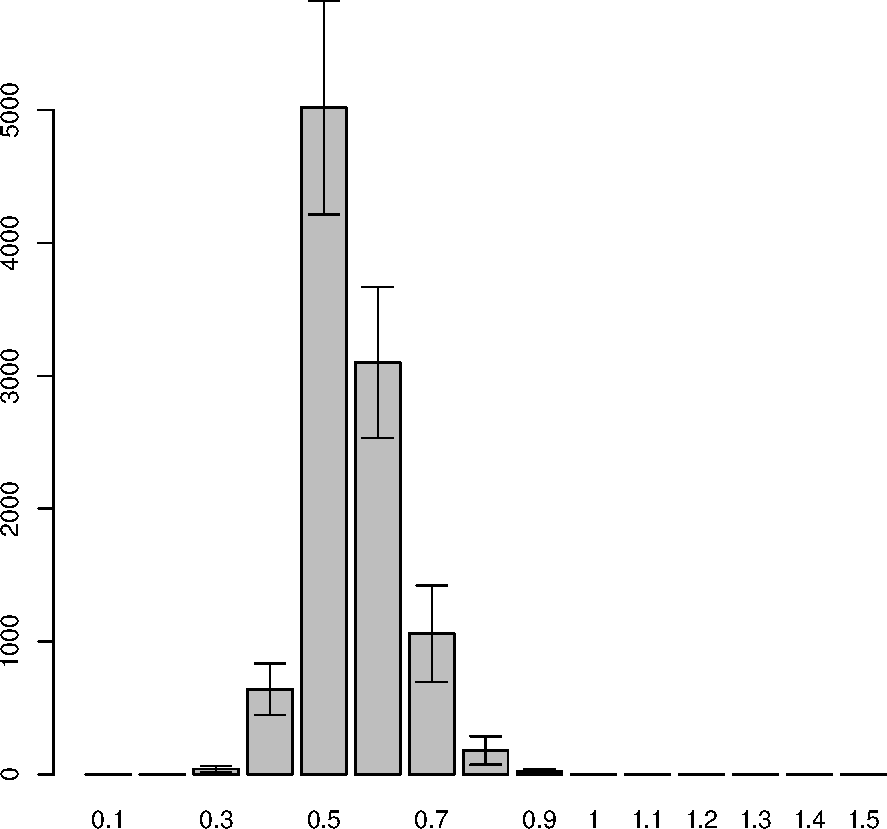
\includegraphics[width=0.215\textheight]{../White_Sea/spat/spat_str_Podpahta_1.pdf}
	\end{center}
	\end{minipage}
		\caption{Размерная стркутура поселений {\it Macoma balthica} на участках в губе Чупа в 2006 году и спата, осевшего в данных поселениях}
		\label{ris:Chupa_spat_sizestr}
\footnotesize{Примечание: по оси абсцисс~--- длина раковины, мм; по оси ординат~--- численность, экз./м$^2$. Планки погрешностей соответсвуют ошибкам средних}
	\end{figure}
Численность спата составляла $4980 \pm 618$~экз./м$^2$. 
Размерная структура спата на данном участке была мономодальная с максимумом при длине раковины $0,6$~мм (рис.~\ref{ris:Chupa_spat_sizestr}).

Численность взрослых моллюсков в Лисьей бухте составляла $1200 \pm 199$~экз./м$^2$, а биомасса "--- $1,9 \pm 0,76$~г/м$^2$. 
На участке были представлены моллюски с раковиной длиной от $1,0$ до $14,3$ мм. 
Размерная структура в Лисьей бухте характеризовалась бимодальностью с модальными классами $1,1 - 3,0$~мм и $8,1 - 10,0$~мм (рис.~\ref{ris:Chupa_spat_sizestr}). 
Численность спата составляла $4040 \pm 832$~экз./м$^2$ (рис. 5). 
Размерная структура спата на данном участке была мономодальная с максимумом при длине раковины $0,5$~мм (рис.~\ref{ris:Chupa_spat_sizestr}).

Численность взрослых маком на участке в бухте Клющиха составляла $476 \pm 291$~экз./м$^2$, а биомасса "--- $1,1 \pm 0,27$~г/м$^2$. 
На участке были представлены моллюски с раковиной длиной от $1,3$ до $11,5$~мм. 
Размерная структура в бухте Клющиха характеризовалась бимодальностью с модальными классами $1,1 - 2,0$~мм и $6,1 - 8,0$~мм (рис.~\ref{ris:Chupa_spat_sizestr}). 
Численность спата составляла $4240 \pm 441$~экз./м$^2$. 
Размерная структура спата на данном участке была мономодальная с максимумом при длине раковины $0,75$~мм (рис.~\ref{ris:Chupa_spat_sizestr}).

Численность {\it M.~balthica} в проливе Подпахта составляла $228 \pm 69$~экз./м$^2$, а биомасса "--- $1,9 \pm 1,21$~г/м$^2$. 
На участке были представлены моллюски с раковиной длиной от $1,1$ до $13,5$~мм. 
Размерная структура на участке в проливе Подпахта характеризовалась бимодальностью с модальными классами $1,1 - 2,0$~мм и $9,1 - 10,0$~мм (рис.~\ref{ris:Chupa_spat_sizestr}). 
Численность спата составляла $10060 \pm 1493$~экз./м$^2$. 
Размерная структура спата на данном участке была мономодальная с максимумом при длине раковины $0,5$~мм (рис.~\ref{ris:Chupa_spat_sizestr}).

Для выявления связи численности спата с обилием (численностью и биомассой) взрослых маком был рассчитан ранговый коэффициент корреляции Спирмена (табл.~\ref{spat_abult_correlation}). 
\begin{table}[p]
\caption{Корреляция численности спата M. balthica с  обилием взрослых маком в поселениях}
\label{spat_abult_correlation}
\begin{center}
\begin{tabular}{|l|lll|}
\hline
     & $r_S$    & $t_{N-2}$   & $p$    \\ \hline
$N_{ad}$ & -0,46 & -2,209 & 0,04 \\
$B_{ad}$ & -0,05 & -0,214 & 0,83\\ \hline
\end{tabular}
\end{center}

\footnotesize{Примечание: $N_{ad}$ --- средняя численность взрослых маком в поселении; 
$B_{ad}$ --- средняя биомасса взрослых маком в поселении; 
$r_S$ --- значение рангового коэффициента корреляции Спирмена; 
$t_{N-2}$ --- критерий Стьюдента;   
$p$ --- уровень значимости нулевой гипотезы.}
\end{table}
До\-сто\-вер\-ная корреляция ($r_S = -0,46$) была показана между численностью спата и средней численностью взрослых маком в поселении, в то время как корреляция количества спата со средней биомассой взрослых особей оказалась недостоверной.

Также был рассчитан ранговый коэффициент корелляции Спирмена для обилия спата и средней численности отдельных размерных групп взрослых маком. 
Для этого были выделены размерные группы с шагом $3$~мм (рис.~\ref{ris:spearman_size},~А).
	\begin{figure}[p]
	\begin{minipage}[b]{.46\linewidth}
	\begin{center}
	А
	\end{center}
	\end{minipage}
	%
	\hfil %Это пружинка отодвигающая рисунки друг от друга
	\begin{minipage}[b]{.46\linewidth}
	\begin{center}
	Б
	\end{center}
	\end{minipage}
	\begin{minipage}[b]{.46\linewidth}
%Фигурка в первом ряду слева размер отведенный под весь этот объект \textendash 0.46 от ширины строки
%Параметр [b] означает, что выравнивание этих министраниц будет по нижнему краю
	\begin{center}
		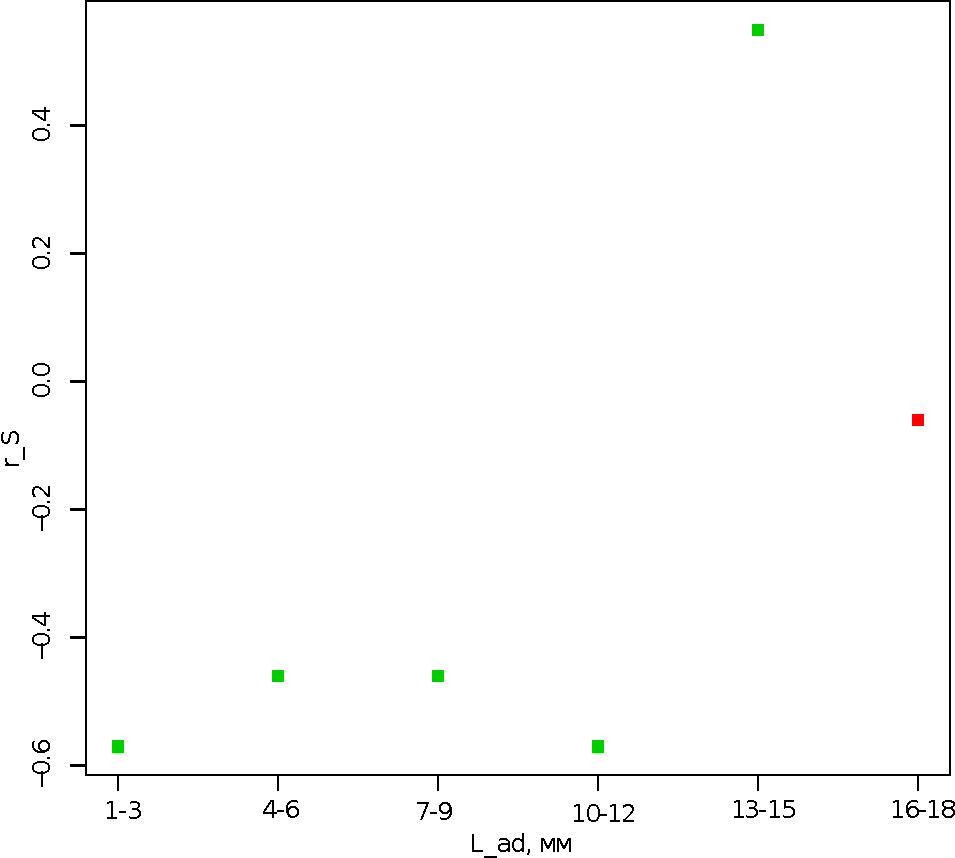
\includegraphics[width=\textwidth]{../White_Sea/spat/spearman_spat_3mm_1.pdf}
	\end{center}
	\end{minipage}
%
	\hfil %Это пружинка отодвигающая рисунки друг от друга
	\begin{minipage}[b]{.46\linewidth}
%Фигурка в первом ряду слева размер отведенный под весь этот объект \textendash 0.46 от ширины строки
%Параметр [b] означает, что выравнивание этих министраниц будет по нижнему краю
	\begin{center}
		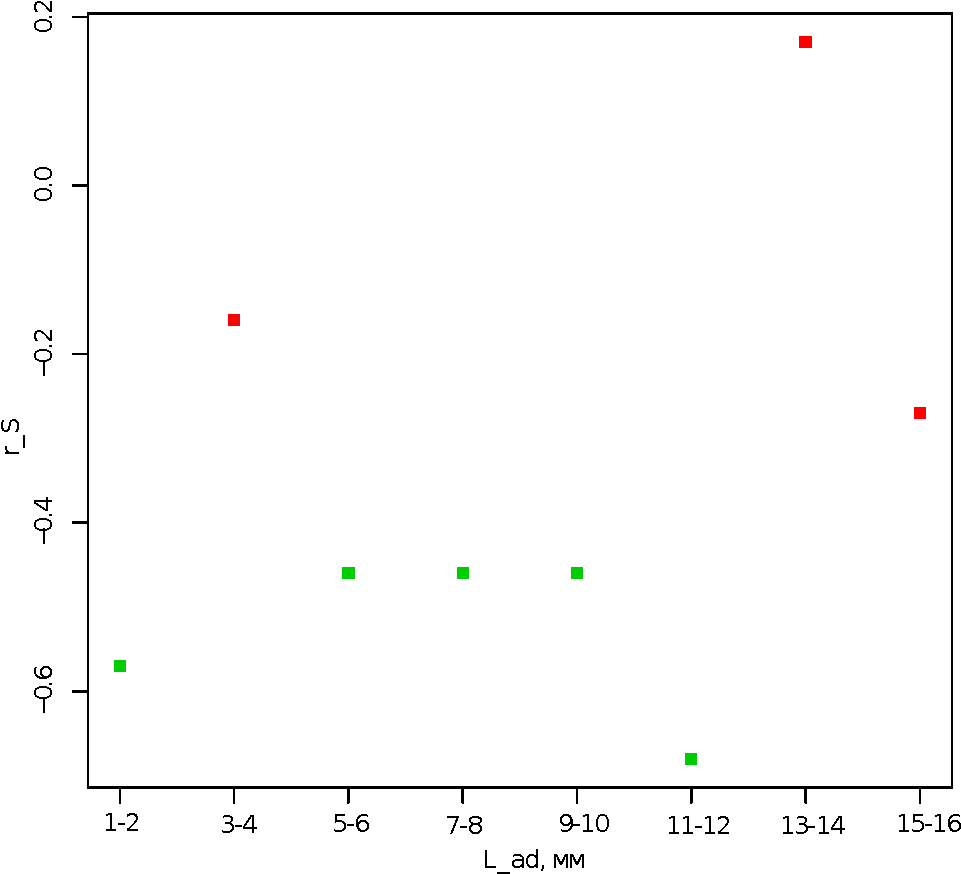
\includegraphics[width=\textwidth]{../White_Sea/spat/spearman_spat_2mm_1.pdf}
	\end{center}
	\end{minipage}
	\caption{Изменение силы и характера корреляции численности спата с численностью взрослых особей в поселениях, с учетом размерной характеристики последних}
	\label{ris:spearman_size}
	
	\footnotesize{Примечание: $r_S$ – значение рангового коэффициента корелляции Спирмена;
 $L_{ad}$ – длина взрослых особей,~мм. \\
Зеленые точки --- достоверные коэффициенты при $p \le 0,05$}
	\end{figure}
Достоверный отрицательный коэффициент корреляции ($-0,46 - -0,57$) был показан для маком длиной до $12$~мм, при этом максимальная корреляция ($-0,57$) достигалась дважды: для групп $1-3$~мм и $9-12$~мм. 
Достоверная положительная корреляция ($r_S=0,55$) была показана между обилием спата маком и численностью взрослых особей длиной $12-15$~мм.

Однако при расчете аналогичного показателя при разделении взрослых особей на классы с шагом $2$~мм, если первая группа (особи длиной менее $12$~мм) также достоверно коррелирует с численностью спата, то группа $12-14$~мм, хотя и положительно коррелирует, но эта связь уже не достоверна (рис.~\ref{ris:spearman_size},~Б).

Поскольку объем выборки небольшой, то мощность корреляционного анализа невелика. 
Поэтому для оценки влияния численности взрослых маком на размеры пополнения был проведен дисперсионный анализ и оценена сила влияния факторов (табл.~\ref{tab:ANOVA_site_Nad_spat}).
Поскольку невозможно изолировать влияние условий на локальном участке и анализировать влияние только численности взрослых маком, то была выбрана иерархическая схема дисперсионного анализа, в которой фактор <<участок>> был вложен в фактор <<численность крупных маком>>.
\begin{table}[p]
\caption{Анализ структуры вариансы (иерархический дисперсионный анализ) показателей численности спата маком в градиентах плотности взрослых маком в поселениях и местоположения участка}
\label{tab:ANOVA_site_Nad_spat}
\begin{center}
\begin{tabular}{|l|lll|ll|ll|ll|}
\hline
                & $SS$        & $df$ & $MS$       & $F$      & $p$        & $\nu^2$      & $m_{\nu^2}$       & $F_{\nu^2}$            & $F_{cr}$  \\ \hline
  site($N_{ad}$) & 86890000  & 2  & 43445000 & 9,9326 & 0,0016 & 0,45 & 0,068 & 6,63 & 3,63 \\
$N_{ad}$         & 34848000  & 1  & 34848000 & 7,9671 & 0,0123 & 0,18 & 0,051 & 3,55 & 4,49 \\
error       & 69984000  & 16 & 4374000  &        &          &              &              &              &      \\ \hline
\end{tabular}
\end{center}

\footnotesize{Примечание: Источник вариации: $N_{ad}$ --- фактор <<численность взрослых особей>>, 
site ($N_{ad}$) --- фактор <<участок>> (вложен в фактор $N_{ad}$),
error ---  внутригрупповая вариация. \\
$SS$ --- девиата, 
$df$ --- число степеней свободы, 
$MS$ --- варианса, 
$F$ --- значение критерия Фишера, 
$p$  --- уровень значимости,
$\nu^2$ --- сила влияния фактора,
$m_{\nu^2}$ --- ошибка силы влияния,
$F_{\nu^2}$ – значение критерия Фишера для силы влияния.}
\end{table}
По результатам дисперсионного анализа как численность взрослых особей, так и уникальный набор условий каждого участка достоверно влияют на количество маком, осевших в поселении, причем вариабельность от участка к участку выше, чем вариабельность, обусловленная высокой или низкой численностью взрослых особей в поселении. 
%Однако достоверно оценить силу влияния возможно только для фактора <<участок>>.

Также исследованные участки отличались по суммарному обилию макрозообентоса (табл.~\ref{tab:NB_fauna_spat}). 
	\begin{table}[p]
	\caption{Характеристики общего обилия макрозообентоса  на участках в губе Чупа в 2006 году}
	\label{tab:NB_fauna_spat}
	\begin{center}
		\begin{tabular}{|l|c|c|}
		\hline
		                & $N_f$, экз./м$^2$ (d, \%) & $B_f$ г/м$^2$ (d, \%)      \\ \hline 
		Сухая салма     & 9381 (12,7) & 141,7 (12,3) \\
		Лисья губа      & 42544 (11,2) & 151,3  (11,3) \\
		бухта Клющиха   & 1344 (19,1) & 37,8 (34,2) \\
		пролив Подпахта & 7169 (28,4) & 46,6 (19,4) \\ \hline
		\end{tabular}
	\end{center}

\footnotesize{Примечание: $N_f$ --- средняя суммарная численность макробентоса в поселении,~экз./м$^2$; $B_f$ --- средняя суммарная биомасса макробентоса в поселении,~г/м$^2$. В скобках приведена точность учета (в \%)}
	\end{table}
Наименьшее обилие макрозообентоса было отмечено на участке в бухте Клющиха ($N = 1344 \pm 256,2$~экз./м$^2$; $B = 37,8 \pm 12,9$~г/м$^2$). 
Б\'{o}льшие численности были отмечены в Сухой Салме ($N = 9381 \pm 2678$~экз./м$^2$) и проливе Подпахта ($N = 7169 \pm 4545$~экз./м$^2$), но различия между этими участками недостоверное. 
Однако по биомассе макрозообентоса участок в Сухой Салме на порядок отличается от пролива Подпахта ($B = 147,1 \pm 17,3$~г/м$^2$ и $46,6 \pm 9,0$~г/м$^2$, соответственно). 
Максимальное обилие макробентоса отмечено на участке в бухте Лисьей, где численность ($42544 \pm 4753,4$) достоверно отличается от всех других участков, а биомасса достоверно больше, чем в проливе Подпахта и бухте Клющиха, но не отличается от аналогичного показателя в Сухой Салме.

Для выявления связи численности и биомассы макрозообентоса с численностью спата {\it M.~balthica} был рассчитан ранговый коэффициент корреляции Спирмена (табл.~\ref{spat_fauna_correlation}). 
\begin{table}[p]
\caption{Корреляция численности спата M. balthica с обилием макробентоса в поселениях}
\label{spat_fauna_correlation}
\begin{center}
\begin{tabular}{|l|lll|}
\hline
     & $r_S$    & $t_{N-2}$   & $p$    \\ \hline
$N_{fauna}$  & -0,16 & -0,68 & 0,50 \\
$B_{fauna}$  & -0,16 & -0,68 & 0,50\\
\hline
\end{tabular}
\end{center}

\footnotesize{Примечание: $N_{fauna}$ --- средняя численность взрослых маком в поселении; 
$B_{fauna}$ --- средняя биомасса взрослых маком в поселении; 
$r_S$ --- значение рангового коэффициента корреляции Спирмена; 
$t_{N-2}$ --- критерий Стьюдента;   
$p$ --- уровень значимости нулевой гипотезы.}
\end{table}
Достоверной корреляции между численностью спата макомы с суммарными численностью и биомассой макрозообентоса обнаружено не было.


\bigskip
Таким образом, оседание спата широко варьирует в пределах локальных акваторий.
Причем уникальное сочетание условий, характерных для каждого поселения, то есть локальный участок, оказывает значительное влияние на численность спата.
В то же время удалось показать влияние численности крупных маком на величину оседания.


\afterpage{\clearpage}
